% -----------------------------------------------
% Template for SMC 2020
% adapted from previous SMC paper templates
% -----------------------------------------------

\documentclass{article}
\usepackage{smc2020}
\usepackage{times}
\usepackage{ifpdf}
\usepackage[english]{babel}
\usepackage{cite}

%%%%%%%%%%%%%%%%%%%%%%%% Some useful packages %%%%%%%%%%%%%%%%%%%%%%%%%%%%%%%
%%%%%%%%%%%%%%%%%%%%%%%% See related documentation %%%%%%%%%%%%%%%%%%%%%%%%%%
%\usepackage{amsmath} % popular packages from Am. Math. Soc. Please use the 
%\usepackage{amssymb} % related math environments (split, subequation, cases,
%\usepackage{amsfonts}% multline, etc.)
%\usepackage{bm}      % Bold Math package, defines the command \bf{}
%\usepackage{paralist}% extended list environments
%%subfig.sty is the modern replacement for subfigure.sty. However, subfig.sty 
%%requires and automatically loads caption.sty which overrides class handling 
%%of captions. To prevent this problem, preload caption.sty with caption=false 
%\usepackage[caption=false]{caption}
%\usepackage[font=footnotesize]{subfig}


%user defined variables
\def\papertitle{SEAM PROJECT - SUSTAINED STEREOPHONY}
\def\firstauthor{Giuseppe Silvi}
\def\secondauthor{Davide Tedesco}
\def\thirdauthor{Third author}

% adds the automatic
% Saves a lot of output space in PDF... after conversion with the distiller
% Delete if you cannot get PS fonts working on your system.

% pdf-tex settings: detect automatically if run by latex or pdflatex
\newif\ifpdf
\ifx\pdfoutput\relax
\else
   \ifcase\pdfoutput
      \pdffalse
   \else
      \pdftrue
\fi

\ifpdf % compiling with pdflatex
  \usepackage[pdftex,
    pdftitle={\papertitle},
    pdfauthor={\firstauthor, \secondauthor, \thirdauthor},
    bookmarksnumbered, % use section numbers with bookmarks
    pdfstartview=XYZ % start with zoom=100% instead of full screen; 
                     % especially useful if working with a big screen :-)
   ]{hyperref}
  %\pdfcompresslevel=9

  \usepackage[pdftex]{graphicx}
  % declare the path(s) where your graphic files are and their extensions so 
  %you won't have to specify these with every instance of \includegraphics
  \graphicspath{{img/}}
  \DeclareGraphicsExtensions{.pdf,.jpeg,.png}

  \usepackage[figure,table]{hypcap}

\else % compiling with latex
  \usepackage[dvips,
    bookmarksnumbered, % use section numbers with bookmarks
    pdfstartview=XYZ % start with zoom=100% instead of full screen
  ]{hyperref}  % hyperrefs are active in the pdf file after conversion

  \usepackage[dvips]{epsfig,graphicx}
  % declare the path(s) where your graphic files are and their extensions so 
  %you won't have to specify these with every instance of \includegraphics
  \graphicspath{{./figures/}}
  \DeclareGraphicsExtensions{.eps}

  \usepackage[figure,table]{hypcap}
\fi

%setup the hyperref package - make the links black without a surrounding frame
\hypersetup{
    colorlinks,%
    citecolor=black,%
    filecolor=black,%
    linkcolor=black,%
    urlcolor=black
}

\usepackage{color}
\usepackage{listings}
\definecolor{mygrey}{rgb}{0.96,0.96,0.96}
\lstset{
  tabsize=4,
  basicstyle=\ttfamily,
  backgroundcolor=\color{mygrey},
  captionpos=b,
  breaklines=true
}


% Title.
% ------
\title{\papertitle}

% Authors
% Please note that submissions are NOT anonymous, therefore 
% authors' names have to be VISIBLE in your manuscript. 
%
% Single address
% To use with only one author or several with the same address
% ---------------
%\oneauthor
%   {\firstauthor} {Affiliation1 \\ %
%     {\tt \href{mailto:author1@smcnetwork.org}{author1@smcnetwork.org}}}

%Two addresses
%--------------
 \twoauthors
   {\firstauthor} {Affiliation1 \\ %
     {\tt \href{mailto:author1@smcnetwork.org}{author1@smcnetwork.org}}}
   {\secondauthor} {Affiliation2 \\ %
     {\tt \href{mailto:author2@smcnetwork.org}{author2@smcnetwork.org}}}

% Three addresses
% --------------
% \threeauthors
%   {\firstauthor} {Affiliation1 \\ %
%     {\tt \href{mailto:author1@smcnetwork.org}{author1@smcnetwork.org}}}
%   {\secondauthor} {Affiliation2 \\ %
%     {\tt \href{mailto:author2@smcnetwork.org}{author2@smcnetwork.org}}}
%   {\thirdauthor} { Affiliation3 \\ %
%     {\tt \href{mailto:author3@smcnetwork.org}{author3@smcnetwork.org}}}


% ***************************************** the document starts here ***************
\begin{document}
%
\capstartfalse
\maketitle
\capstarttrue
%
\begin{abstract}
\input{abstract.txt}
\end{abstract}
%

\section{Introduction}
\label{sec:introduction}

\emph{Sustained Electro-Acoustic Music} is a project inspired by Alvise Vidolin and Nicola Bernardini's article \cite{bevi05} on \emph{live electroacoustic music sustainability}. In their text, they point at multiple technical faces of the sustainability problem such as technological, notational or general conception issues. Even if the article aforementioned focuses only on \emph{live} electroacoustic music, the concept of sustainability is applicable to any kind of documented music that uses electroacoustic environments including therefore the acousmatic works, instruments mixed with tape and structured amplified works. %This will be the purpose of the presented text.

The main ambition of this project is to grow the interpretation and the electroacoustic musical practice with the consciousness of the electronic and informatics problems that had made arduous to approach this music and prevented the growth of interpretative thinking. It is possible, with a community structure, to determine, build and stratify interpretation of musical core, the repertoire, concealing the environment-related technological issues. They are instruments, not the music itself, after all.

% The process of nota sulla connseguente messa a punto di alcuni principi, eliminando imprecisioni lessicali e formali.

\section{The Seam Community}
\label{sec:seam}

From seam meaning:

\begin{quote}
\begin{it}
A line where two pieces of fabric are sewn together\ldots \\
An underground layer of a mineral such as coal or gold: the buried forests became seams of coal\ldots\\
Join with a seam.
\end{it}
\end{quote}

We have to study Vidolin's gestures to understand Nono, to have a clear sight on our music through an era and join literature and practice with a seam. Vidolin is for Nono what Karajan was for Beethoven: time, consciousness and thinking. We need his work to know what was happening, what we have to do, what is necessary and what doesn't matter. And that is we have to do, seam it just one time, forever. Refine it, maintain it, and again realise it, through practice, forever. Neatly layering people's knowledge and thinking is the only way to hold back and preserve what we are loosing, preventing music from being a boxset of objects without the consciousness of music that they represent. 

To prevent catastrophic regression of musical thinking we must consider that there are few dogmatic concepts to build, re-build and sustain an \emph{electroacoustic repertoire}:
\begin{enumerate}
  \item Open and Be Open
  \item Don't Repeat Yourself
  \item Think and Act as Community
\end{enumerate}

\textbf{SEAM is an Open, DRY, Community.} People inside SEAM will share their knowledge to weld words, papers and literature with meaning.

These are the SEAM organisation coordinates: 
\begin{itemize}
\item \url{http://s-e-a-m.github.io}
\item \url{http://seam-world.slack.com}
\end{itemize}

There are notably predecessors of this kind of initiative, with a more personal oriented use, some of them has inspired this project, like the Miller Puckette's repository\footnote{\url{http://msp.ucsd.edu/pdrp/latest/files/}}. We hope the public domain community profile of SEAM can include some of those precious wizards contributes, in a more community sense, to avoid the misunderstanding of literature. An only-tech reading can bring to wrong interpretations even for great tech minds. That's how Puckette \cite{mp01} resolve a crucial description of the \emph{Dialogue}:

\begin{quote}
This piece in its published form is performed by one clarinetist accompanied by a tape of the same clarinetist.
\end{quote}

It is not accompanied, it is a dialogue. 

%--------------------------------------------------------------------------------------------------------------------------------------

\subsection{SEAM Instruments}

Developing the concepts of the instrument and instrumentalist to the combined form of those into interpretation, \cite{lem16,mp01,savi85} requires the overcoming of obsolete parallelism: the computer music performer as an artisan of \emph{new-luthiery}. There is not a sustainability conception under the deception of that wrong and obsolete metaphor. Each \emph{luthiery} is new, it evolve with musical needs. Each instrument has his inventor and his virtuoso, but in musical history, those people never coincided. The best instruments were conceived from men entirely devoted to the conception of something unique. The best virtuoso took those instruments to unveil their prospective.

%\begin{quote}
%For computer music, things are slightly different because of the nature of the “instrument”. There is an extra step: constructing the instrument. In this sense the computer music performer is also his own instrument-builder (luthier). Moreover, there is no school or conservatory to learn how to become a computer virtuoso today.
%\end{quote}

During the lessons in Rome Conservatory in which \emph{SEAM} was born and its related problems were shared with classes to sensitize students to community work, the core software used to explode issues was \emph{Faust}\footnote{\url{https://faust.grame.fr}}. This wasn't a restriction, it was a preference. Text-based DSP offers the deepest learning experience and great expressivity and readability. \emph{Faust} code could be written to educate a musician at the same time with computation versatility and efficiency. The \emph{Faust libraries} concept is useful to focus on write once, and read forever, code. We think \emph{Faust} itself represents a rather concept of electroacoustic sustainability. Thinking, for example, at the \emph{filters.lib} and at the names that contributed the enrichment of speculation around each object, make us wish to a musical interest capable to do community more than with the adoption of other software.

Instruments carved by musical ideas on readable text (code) becomes a sub-literature in which each brick maintain the power of the source code, the clarity of an equation, the efficiency of the continuous development, the reusability of a word in different contexts. 

%--------------------------------------------
%----------------larghezza massima del codice
\begin{lstlisting}
import("stdfaust.lib");
import("../faust-libraries/seam.lib");
\end{lstlisting}

The \emph{SEAM library} local importing points to other libraries catalogued by arguments, like in \emph{Standard Faust Libraries}. 

Actually there are five different libraries:
\begin{description}
  \item[seam.lib] contains general functions and the pointers to each specific library. It may also comprehend the custom performative environment definition, as it could be for the inputs and the outputs, the setup parameters and the performative controls.
  \item[gerzon.lib] contains early Michael Gerzon works, his core concepts of spatialization and stereophony, that conducted him to conceive the Ambisonic technology. In a sustained environment, the role of this library is to avoid misunderstanding of what \emph{stereo} is \cite{ab58} and what we are loosing in the electroacoustic staging perception. 
  \item[hardware.lib] contains hardware-related functions like MIDI mapping and I/O assignment to an audio interface, with a routing strategy to connect instruments to real-world hardware with a graphical user interface to map routing.
  \item[measurement.lib] contains some audio analysis strategy to define musical display feature for audio inspection, such as integrated measurement and loudness monitoring, that are indispensable tools for today staging of public addressed music.
  \item[nono.lib] is the first author-related library that points to contain \emph{Live Electronics Instruments}. The idea is to collect instruments into the library and use them, work by work, in a hardware-like approach. The \emph{nono.lib} should contain reusable instruments typical of his literature like the Harmonizer, the Halaphon, and so on, directly called back into the performance environment of each work, to enforce the reusability and the sustainability of those instruments. 
\end{description}

Faust is a great tool and we are proud users of it, nevertheless, a studied choose of the proper tool is required for each specific case. Sustaining of proper choosing is most important than the comfort of the preferred tools. As proposed to \emph{max}-addicted students during lessons, a \emph{library} approach, like the \emph{Faust} one, must be ever incentivized.

%--------------------------------------------------------------------------------------------------------------------------------------

\subsection{SEAM Topology}

Referring to the electroacoustic music literature, where the substantial difference with the acoustical one is an inevitable continuously changing of the environment, we prefer to use the topology classification in place of typology one. A typology classification is, according to general type, used where characteristics of something are fixed and produce a catalogue of things. A topology classification considers instead the time-space characteristics of shape and permits the time variance of the environments. We classify three topologies of the electroacoustic music in literature:

\begin{description}
  \item[The undocumented] where composers use only word description to generate environment and circumstances;
  \item[The \emph{words-hole}] where the score has deep technical documentation but listing names of undocumented instruments. Without musicological methodologies, frequently with names without a specific meaning;
  \item[The porting] where informatics translations between languages or informatics technologies are based on literature and shared knowledge.
\end{description}

The identification of topological classes in place of typological forms is necessary to subordinate technology-matter to the musical practice and poetics. %All three topologies are reduced to technological circumstances, not related to the musical content and form, but with the sustainability strategies routes to the music. 

%When we refer to a virtuoso musician, we often point at a violinist or at a piano player: someone who intensely practice on his instrument. This is the central point: Does the violinist builds its own violin every time he approaches a new composition? Does the pianist? The electroacoustic musician does it, every time.

%\section{Floats and equations}
%
%\subsection{Equations}
%Equations should be placed on separated lines and numbered. The number should be on the right side, in parentheses.
%\begin{equation}
%r=\sqrt[13]{3}
%\label{eq:BP}
%\end{equation}
%Always refer to equations like this: ``Equation (\ref{eq:BP}) is of particular interest because...''
%
%\subsection{Figures, Tables and Captions}
%\begin{table}[t]
% \begin{center}
% \begin{tabular}{|l|l|}
%  \hline
%  String value & Numeric value \\
%  \hline
%  Moin! SMC & 2020 \\
%  \hline
% \end{tabular}
%\end{center}
% \caption{Table captions should be placed below the table,  like this.}
% \label{tab:example}
%\end{table}
%
%All artwork must be centered, neat, clean and legible. Figures should be centered, neat, clean
%and completely legible. All lines should be thick and dark enough for purposes of reproduction. Artwork should not be hand-drawn. The proceedings will be distributed in electronic form only, therefore color figures are allowed. However, you may want to check that your figures are understandable even if they are printed in black-and-white.
%
%
%Numbers and captions of figures and tables always appear below the figure/table.
%Leave 1 line space between the figure or table and the caption.
%Figure and tables are numbered consecutively. 
%Captions should be Times 10pt. Place tables/figures in the text as close to the reference as possible, 
%and preferably at the top of the page.
%
%Always refer to tables and figures in the main text, for example: ``see Fig. \ref{fig:example} and \tabref{tab:example}''.
%Figures and tables may extend across both columns to a maximum width of 17.2cm.
%
%Vectorial figures are preferred, e.g., eps. When using \texttt{Matlab}, export using either (encapsulated) Postscript or PDF format. In order to optimize readability, the font size of text within a figure should be no smaller than
%that of footnotes (8~pt font-size). If you use bitmap figures, make sure that the resolution is high enough for print quality. 

\begin{figure}[t]
\centering
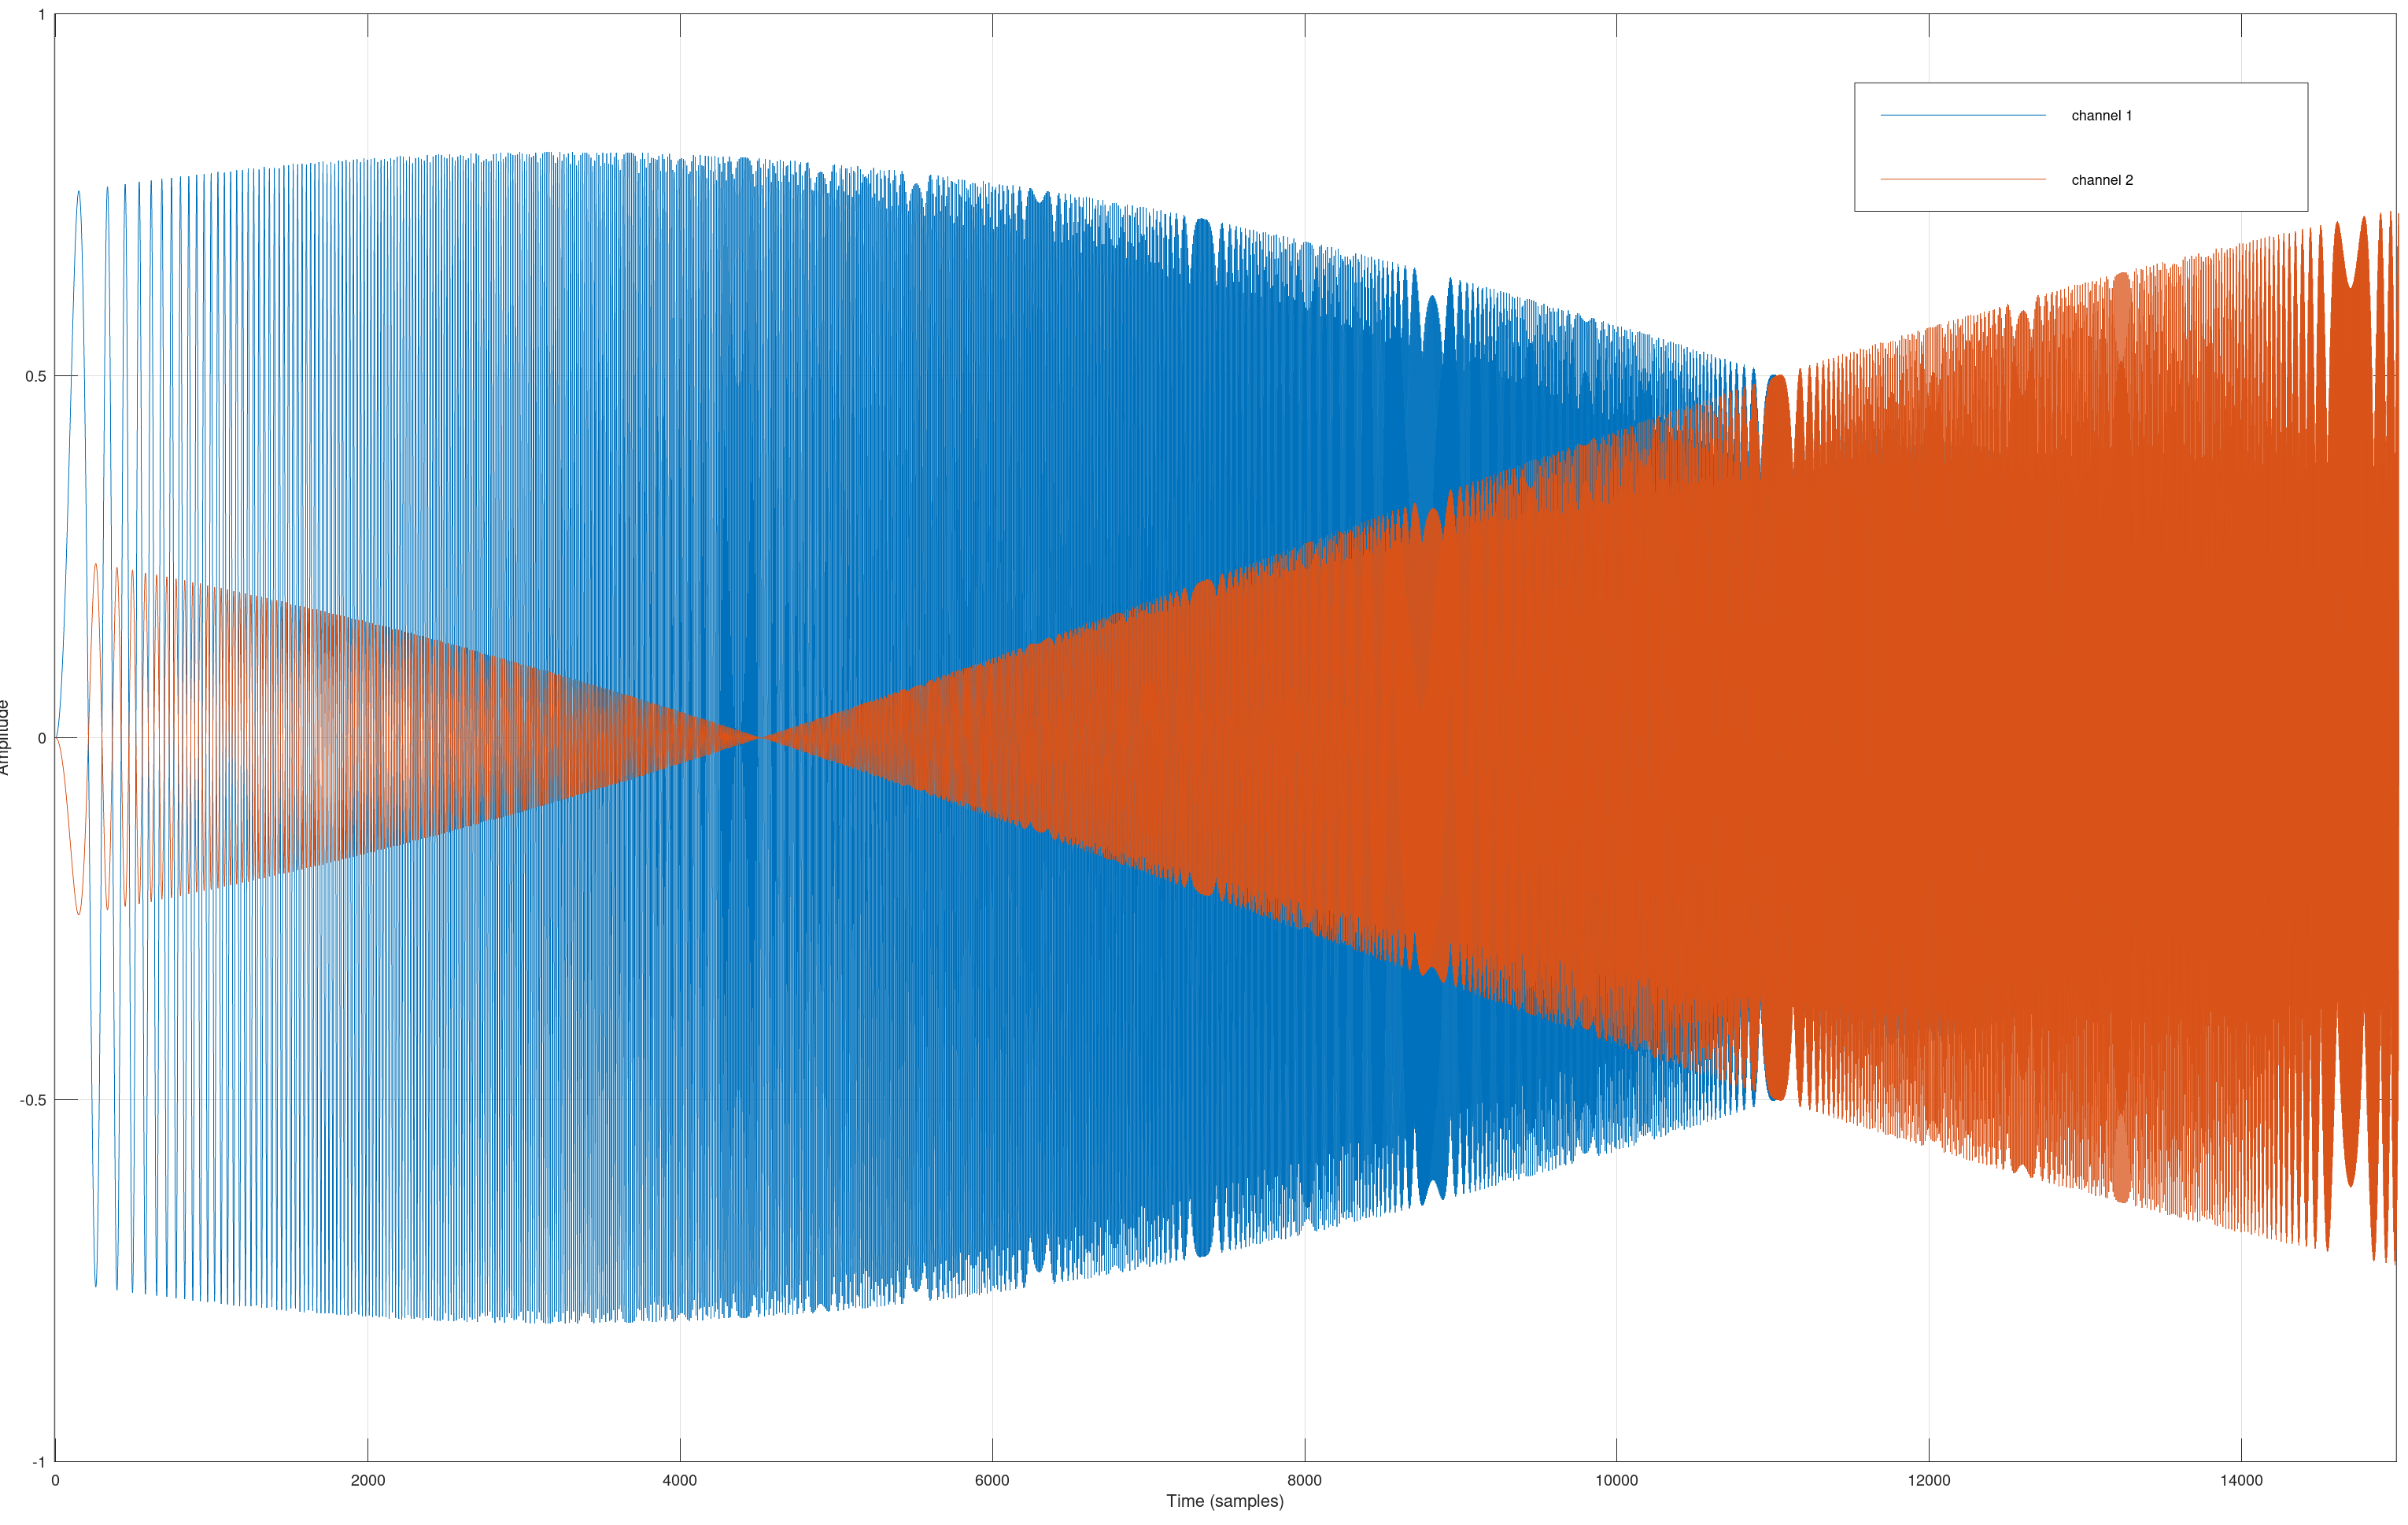
\includegraphics[width=1\columnwidth]{MS2LR-90deg}
\caption{Figure captions should be placed below the figure, 
exactly like this.\label{fig:example}}
\end{figure}

\begin{figure}[t]
\centering
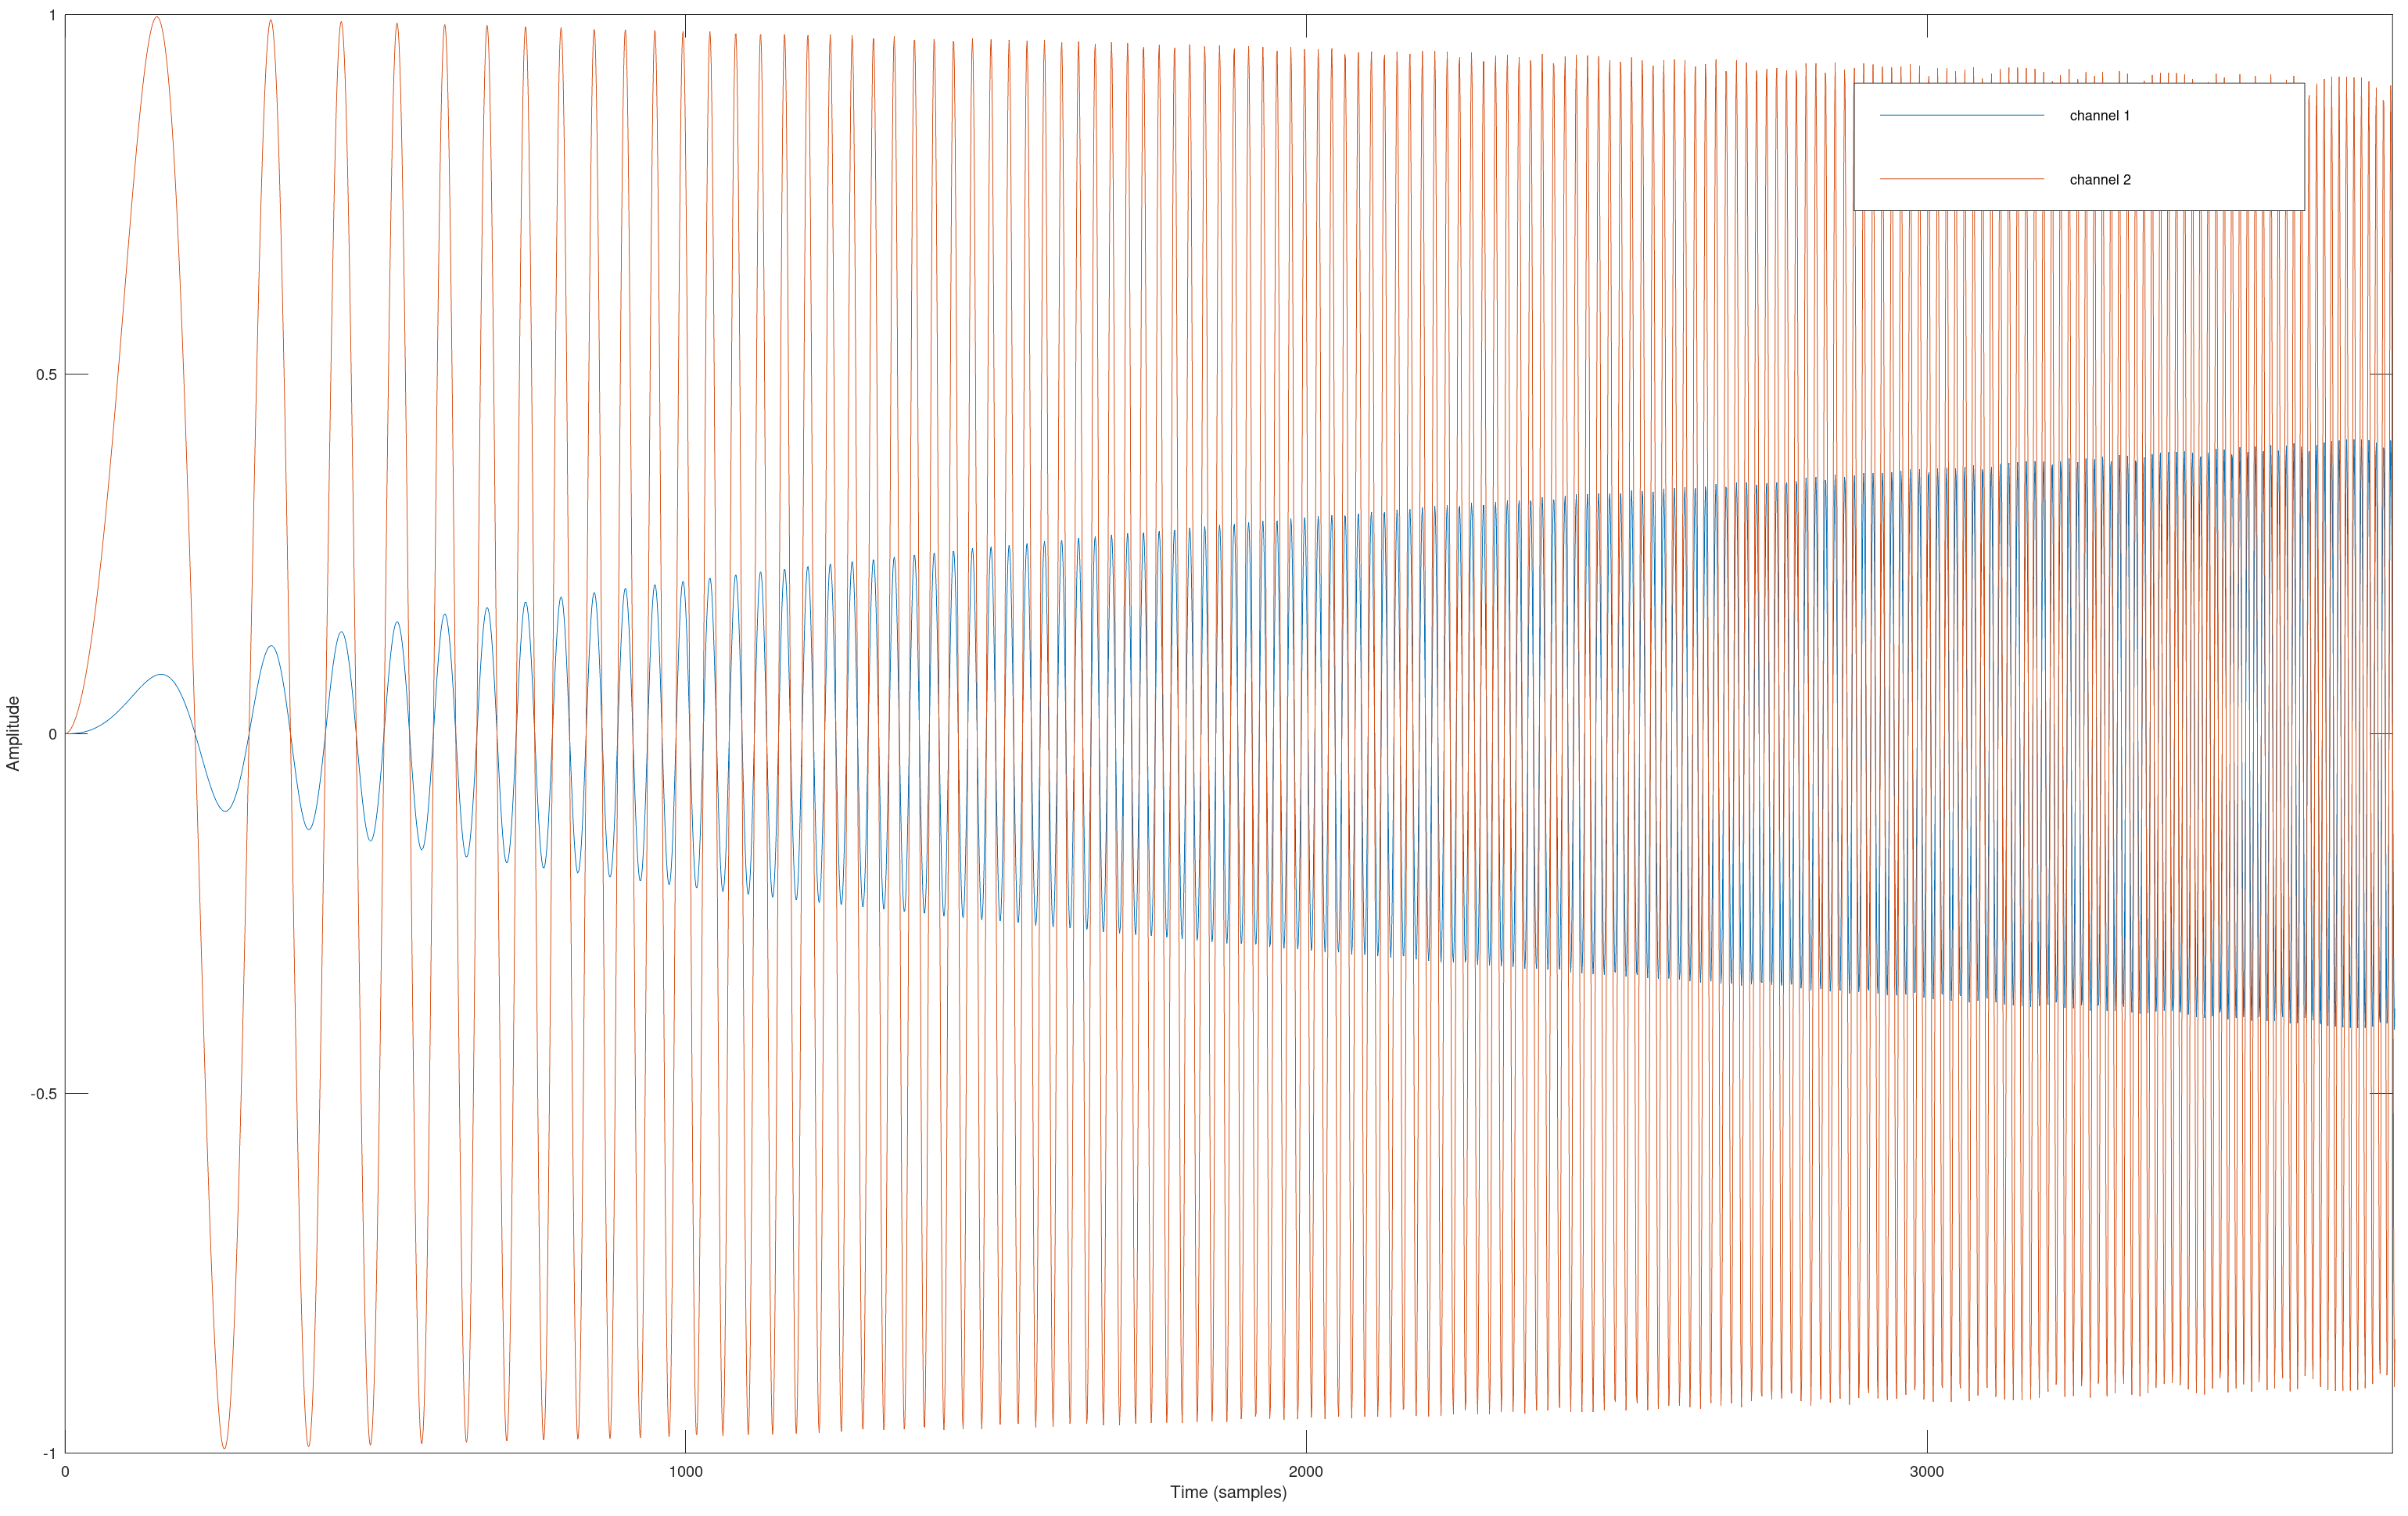
\includegraphics[width=1\columnwidth]{SQRT-LR}
\caption{Figure captions should be placed below the figure, 
exactly like this.\label{fig:example}}
\end{figure}

\begin{figure}[t]
\centering
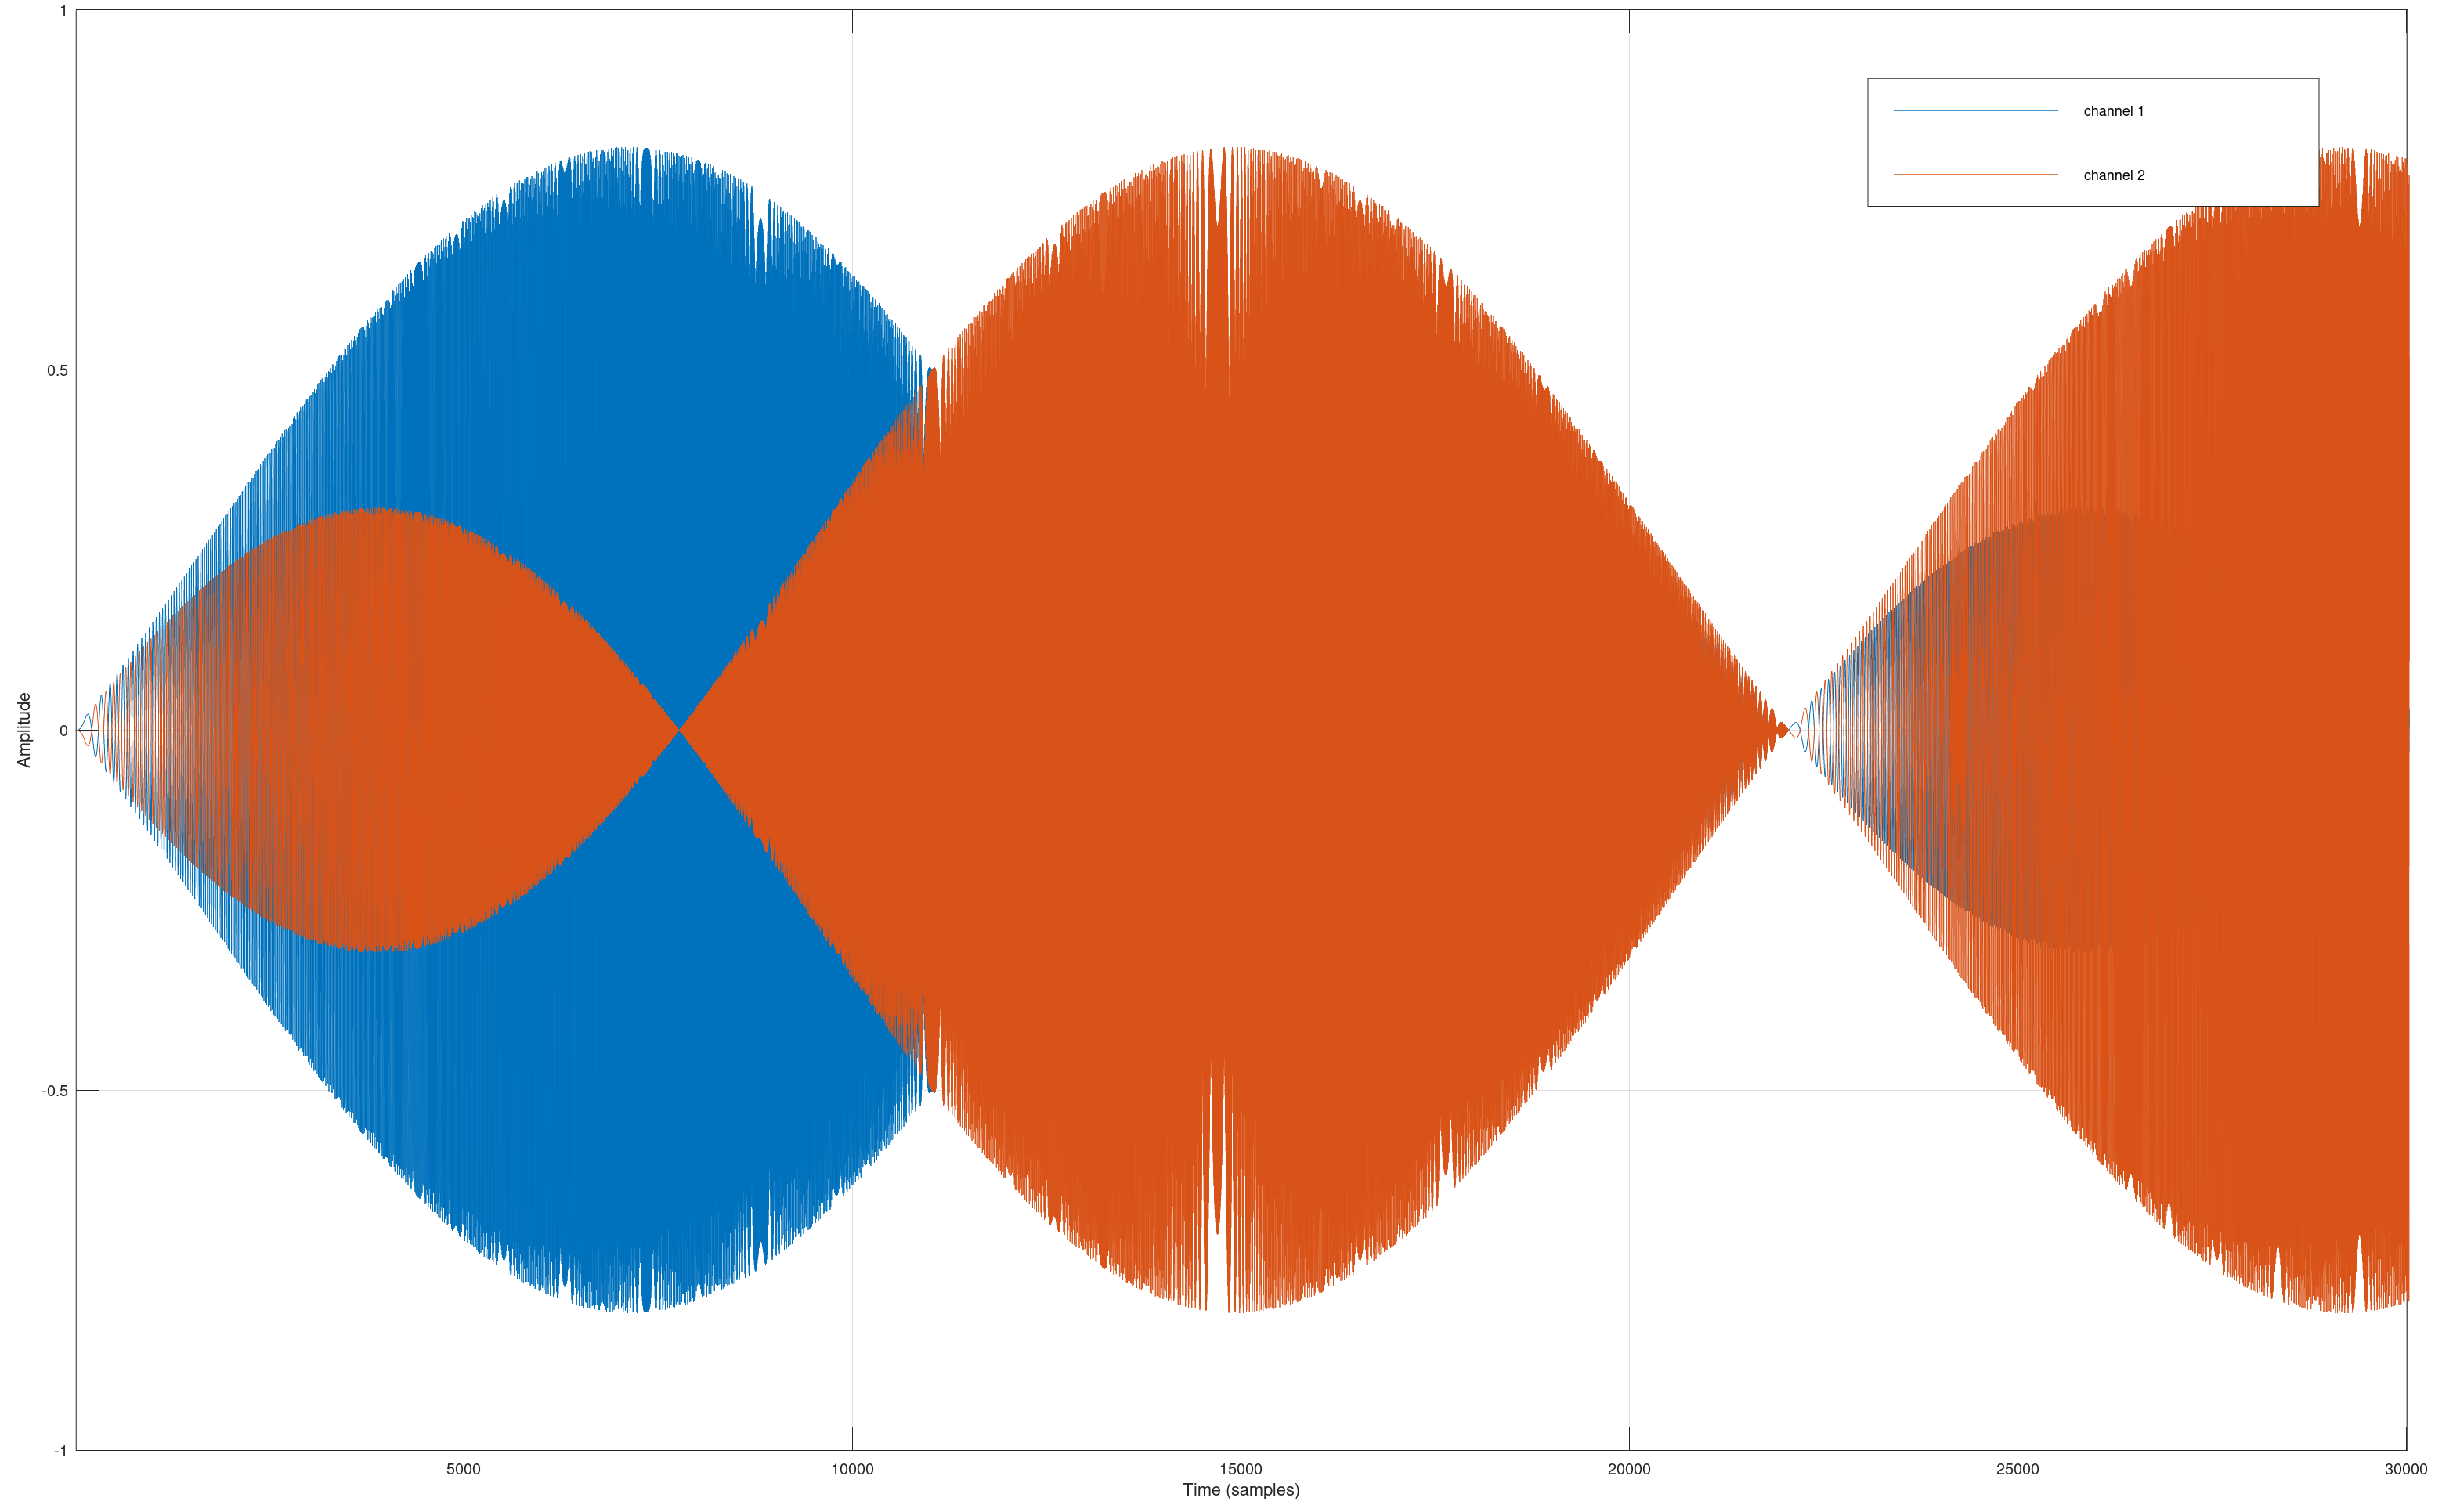
\includegraphics[width=1\columnwidth]{MS2LR-180deg-1}
\caption{Figure captions should be placed below the figure, 
exactly like this.\label{fig:example}}
\end{figure}

\begin{figure}[t]
\centering
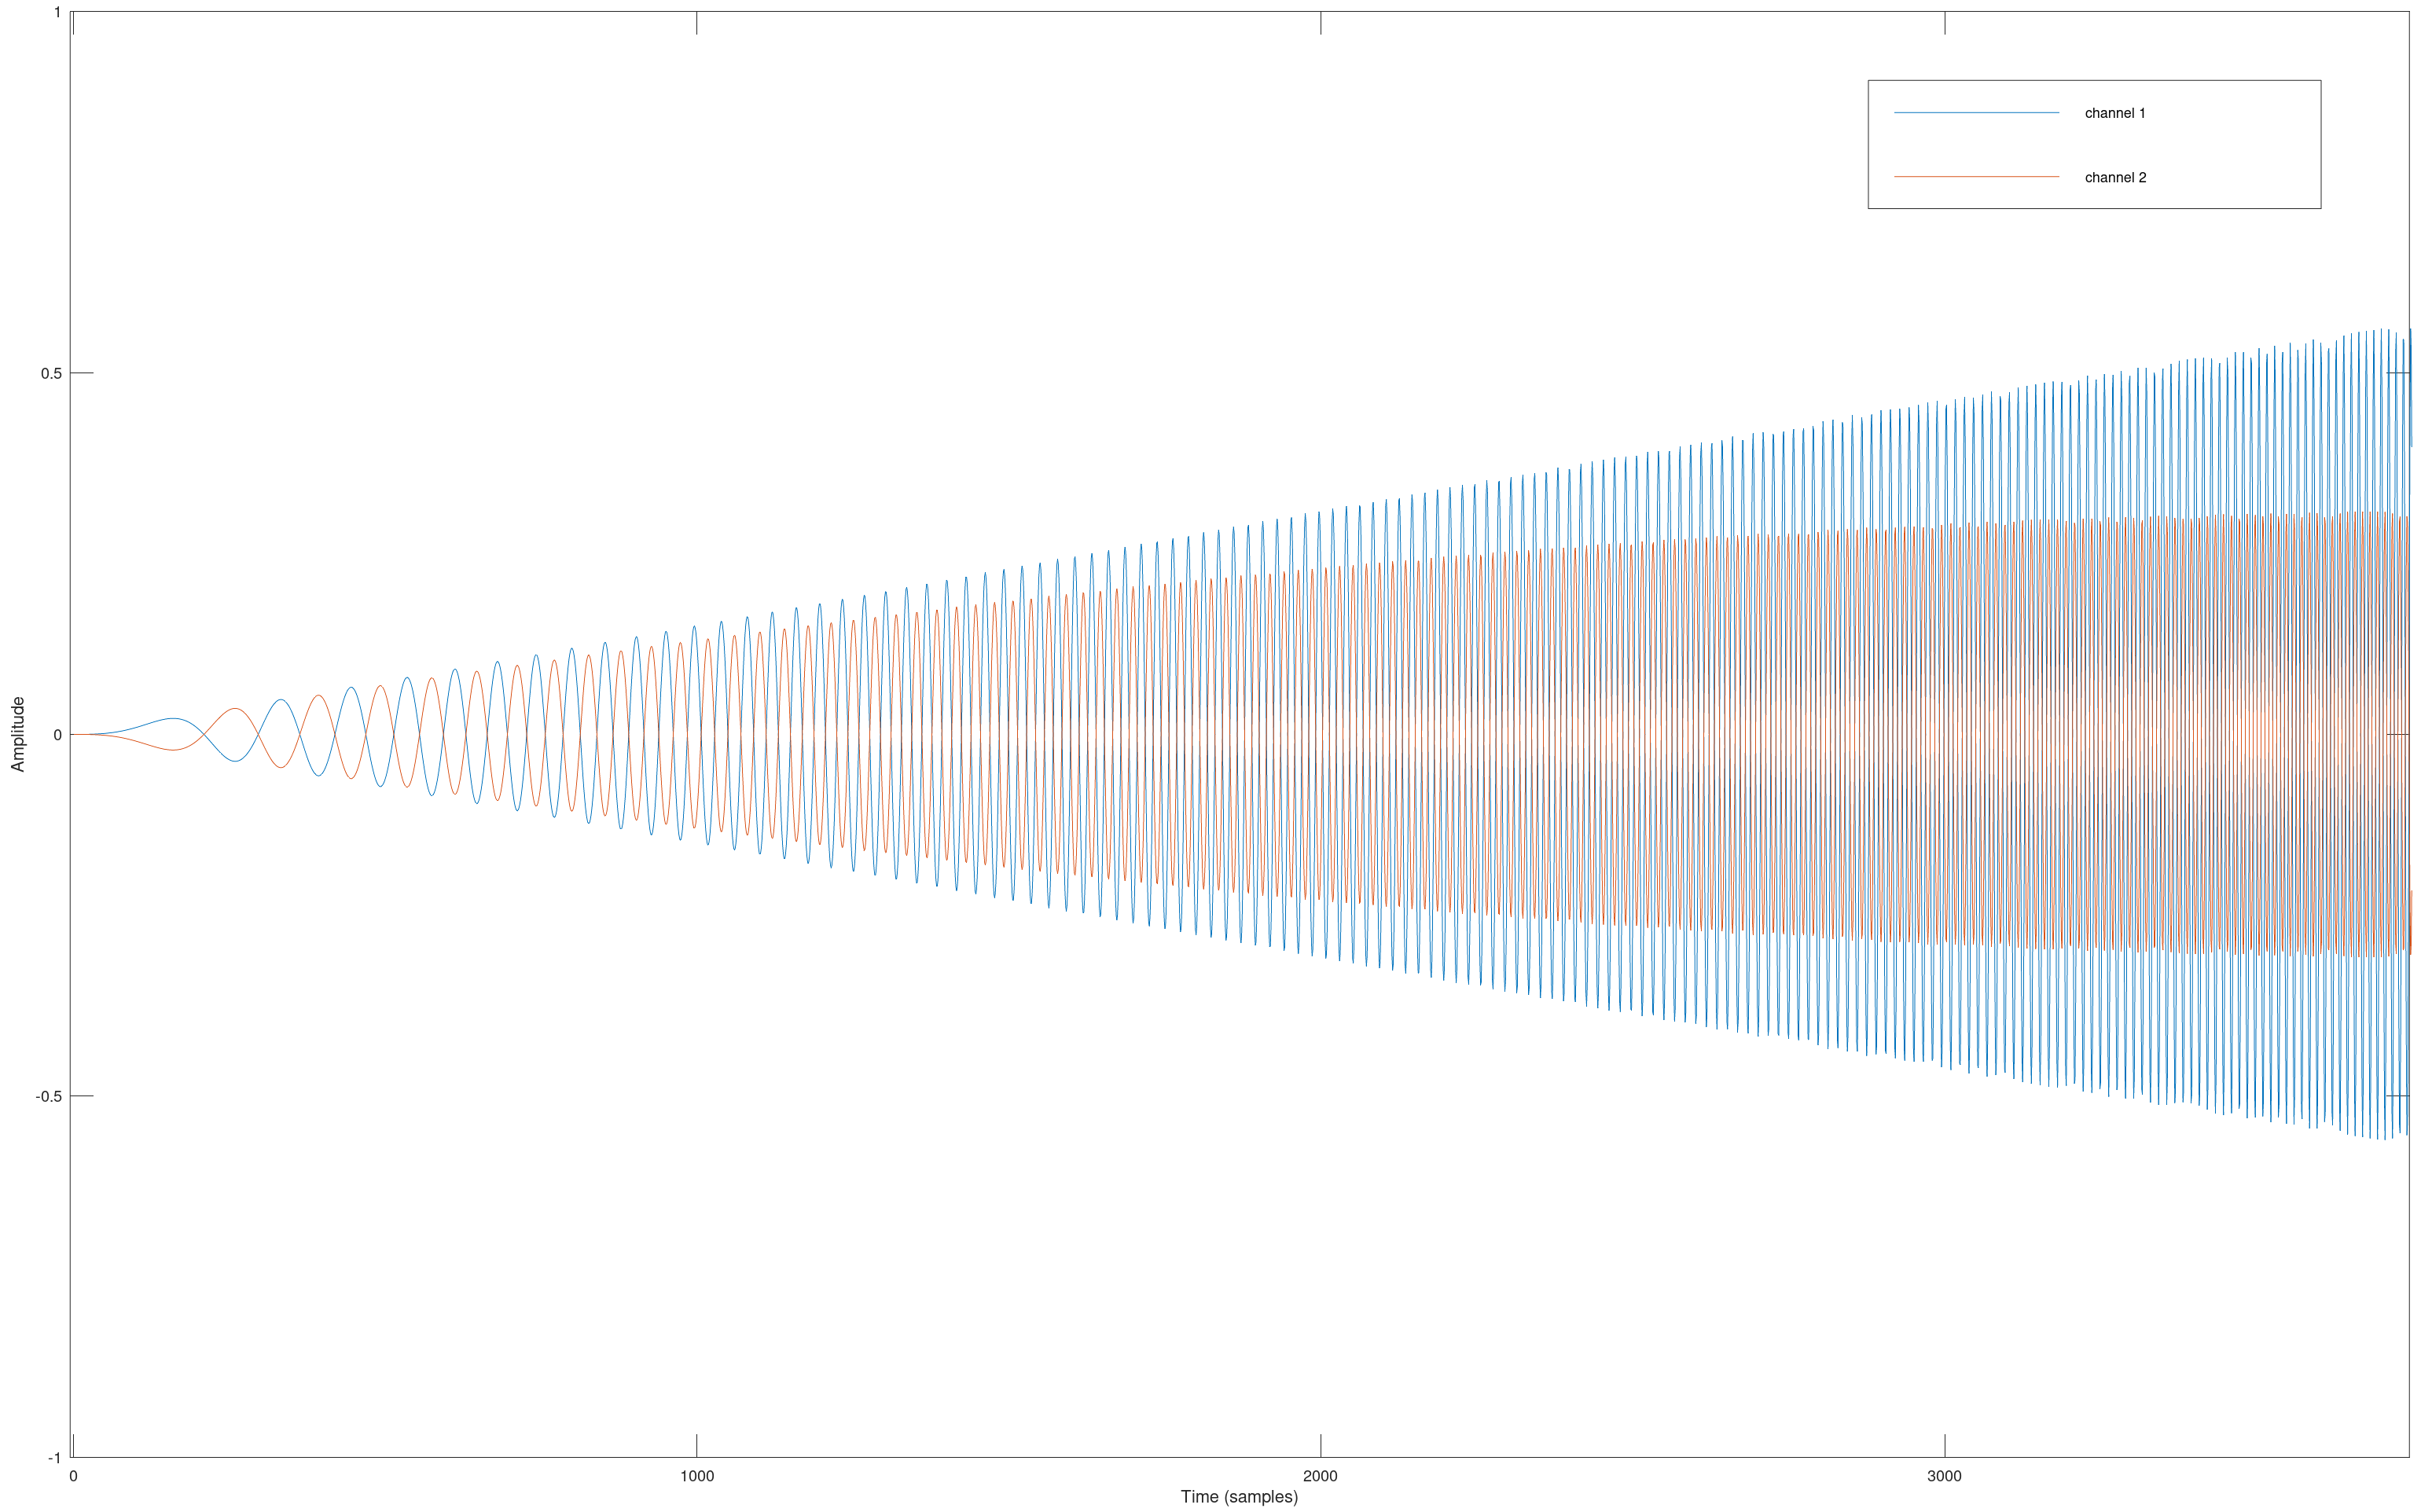
\includegraphics[width=1\columnwidth]{MS2LR-180deg-2}
\caption{Figure captions should be placed below the figure, 
exactly like this.\label{fig:example}}
\end{figure}

\begin{figure}[t]
\centering
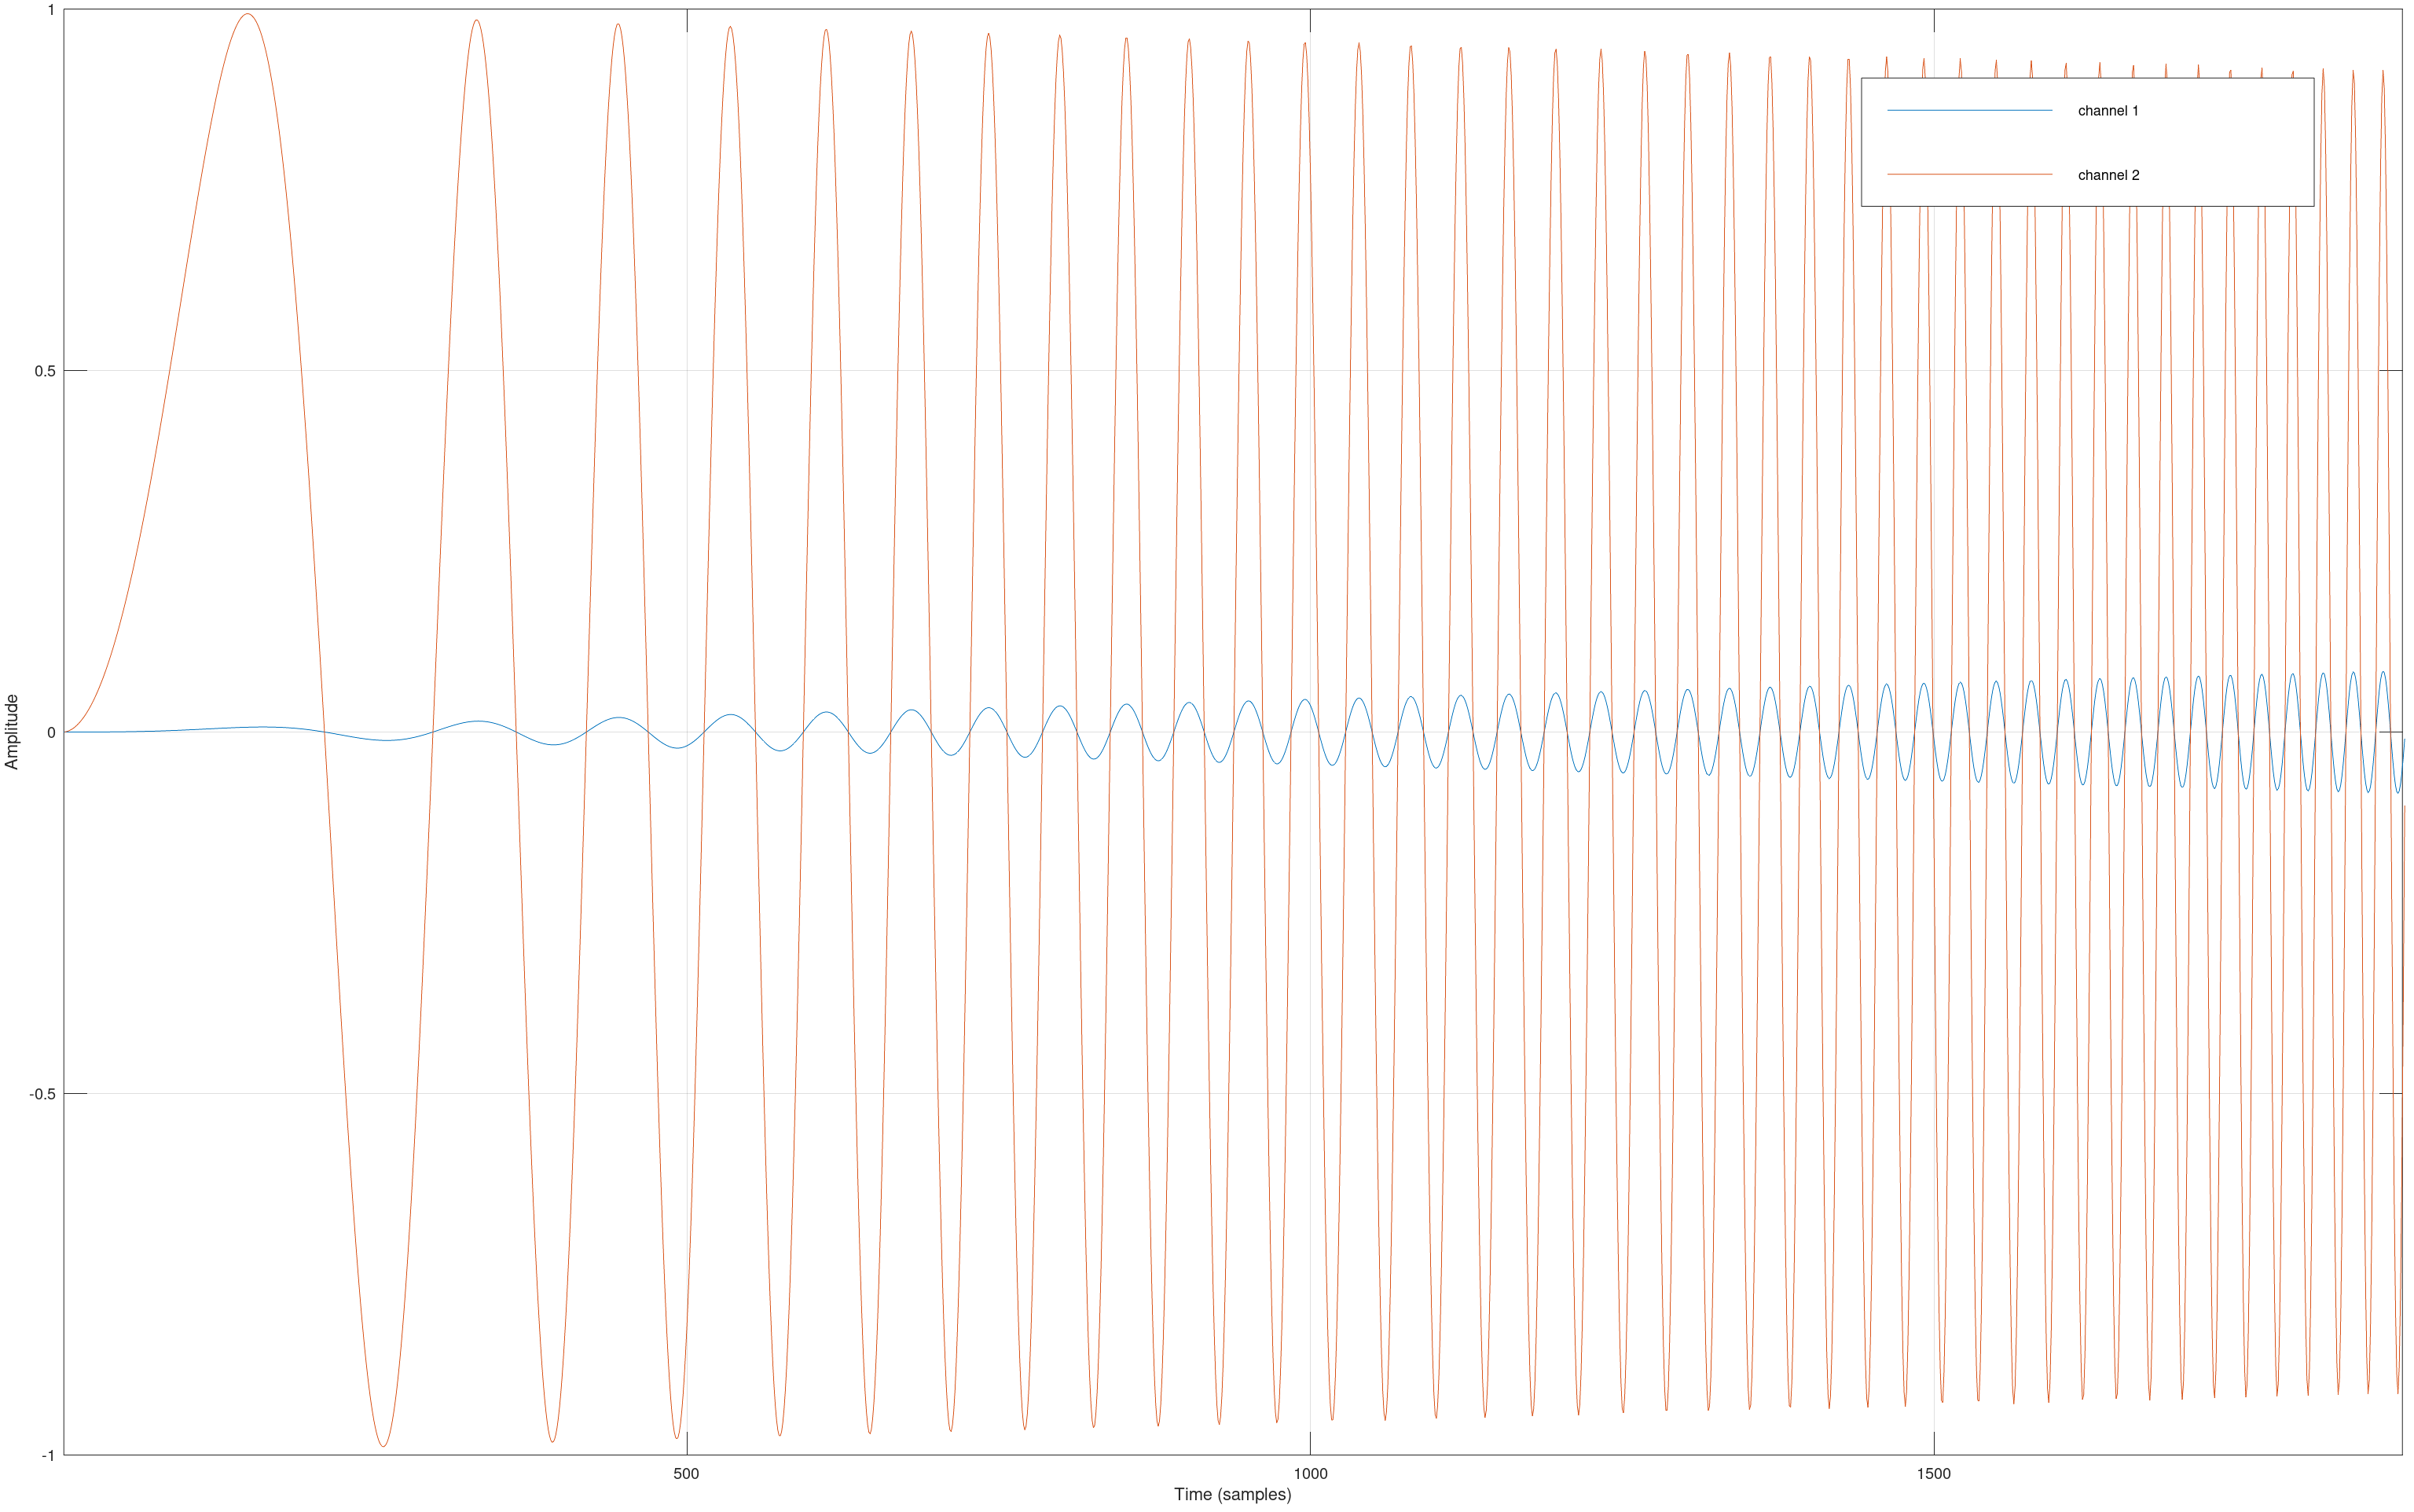
\includegraphics[width=1\columnwidth]{LIN-LR}
\caption{Figure captions should be placed below the figure, 
exactly like this.\label{fig:example}}
\end{figure}

%\section{Citations}
%All bibliographical references should be listed at the end, inside a section named ``REFERENCES''. References must be numbered in order of appearance. You should avoid listing references that do not appear in the text.
%
%Reference numbers in the text should appear within square brackets, such as in~\cite{Someone:00} or~\cite{Someone:00,Someone:04,Someone:09}. The reference format is the standard IEEE one. We highly recommend you use BibTeX 
%to generate the reference list.
%
%\section{Conclusions}
%Please, submit full-length papers. Submission is fully electronic and automated through the Conference Web Submission System. \underline{Do not} send papers directly by e-mail.
%
%
%\begin{acknowledgments}
%At the end of the Conclusions, acknowledgements to people, projects, funding agencies, etc. can be included after the second-level heading  ``Acknowledgments'' (with no numbering).
%\end{acknowledgments} 

%%%%%%%%%%%%%%%%%%%%%%%%%%%%%%%%%%%%%%%%%%%%%%%%%%%%%%%%%%%%%%%%%%%%%%%%%%%%%
%bibliography here
\bibliography{smc2020bib}

\end{document}
